\documentclass[a4paper, 11pt, titlepage]{article}

\usepackage[utf8]{inputenc}
\usepackage{graphicx}
\usepackage{amssymb}
\usepackage{subfig}
\usepackage{amsmath}
\usepackage[pdfborder={0 0 0}]{hyperref}
%\usepackage{fontspec}
%\setmainfont[Mapping=tex-text]{Adobe Garamond Pro}

\begin{document}
\title{Crisis Response in Social Networks}
\author{Joseph F. Harrison \\
        Matthew Revelle \\
        CSS 692, Social Network Analysis \\
        George Mason University}
\date{May 2010}
\maketitle

\tableofcontents

\section{Introduction}
Twitter is a large, social-network platform with a simple premise.  Every user may post short messages and read messages posted by others.  Significant functionality has been built atop Twitter, people share links, photos, videos; participate in conversations, share the geographic coordinates of their current location, and join ad-hoc groups.  Users link themselves with each other by choosing to follow the status updates made by another user.  The follow relationship does not require reciprocity, users Alice and Bob may both follow Carol, but Carol may choose to not follow either of them in return.  In Twitter terminology, Alice and Bob both consider Carol a friend, but Carol does not.  To Carol, Alice and Bob are only followers.

Although the original purpose of posting was to share current status: Alice posts, ``I'm writing a paper about Twitter. Getting hungry.''  Users began to post replies: ``@Alice Take a break if you're hungry, want to grab sushi?''  Messages on Twitter are limited to 140 characters, an artifact of Twitter's original focused support of SMS on mobile phones \cite{Sagolla2009}. The forced brevity inspired compact idioms for denoting metadata.  The ``@''-symbol prefixed to a username is known as a mention.  Mentions signal a user that a message involves them.  Another idiom is the hashtag, a ``\#''-symbol prefixed to a string of characters.  Hashtags mark the message as being related to a particular topic or object, as in ``The humanitarian effort in response of \#haitiquake is ongoing.''

When a user wishes to share a post made by a friend, they may retweet it.  A retweet message includes the text body of the post being retweeted, prefixed with a string that indicates the post is a retweet.  In a post,``RT @Alice A Taste of Burma is delicious!'', the ``RT'' marks the post as a retweet and the immediately following mention of Alice indicates that she is the author of the original post.  Retweeting is commonly used to share interesting statuses from friends with one's own followers; retweeters spread information from their friends to their followers.  In this paper, we use the term \textit{plain tweet} to refer to tweets that are not retweets.

Twitter has previously been used to report and organize a response to emergency situations, such as the crash landing of a plane in the Hudson Bay in January 2009 \cite{Deards2009} and the Iranian 2009 election protest \cite{Grossman2009}.  The research presented in this paper was inspired by those responses, we were interested to better understand how Twitter was used during the aftermath of the Haiti earthquake.

\subsection{Data Summary}
Our analysis focuses on the use of Twitter in the wake of the 2010 earthquake in Haiti. The earthquake struck at 4:53PM local time on 12 January, centered 25km west of Port-au-Prince. We obtained all the tweets pertaining to ``Haiti'' and ``Earthquake'' during the interval, in local time, from 10:21PM, January 12th to 11:54AM, January 13th.  All times in the paper are in UTC unless otherwise noted.  Local time in Haiti is UTC-5, the same offset as EST in the United States.

Our corpus contains 63,196 tweets from 44,430 unique users, with 15,685 retweets and 3,202 replies. The most common hashtag was \textit{\#haiti} with 8,729 occurrences, followed by \textit{\#earthquake} with 3,299, and \textit{\#helphaiti} with 410 occurrences. The dominance of the top two hashtags, shown in Figure~\ref{fig:hashtag_counts}, may be the result of sample bias present in the way this corpus was extracted from the "firehose". For example, if all tweets containing the words "haiti" and "quake" were included it would capture any with those hashtags as well. However, there are 2072 tweets containing neither "haiti" nor "quake" so it's unclear exactly what criteria were used when collecting the corpus.

As visible in Figure \ref{fig:all_tweets_over_time}, Twitter activity drops over night and then surpasses all previous activity frequency in the morning.  There is a noticeable drop in tweet frequency at the end of Figure \ref{fig:all_tweets_over_time}, please note that the last two intervals may be incomplete due to how the data was collected from the Twitter streaming API.

\begin{figure}[h]
\centering
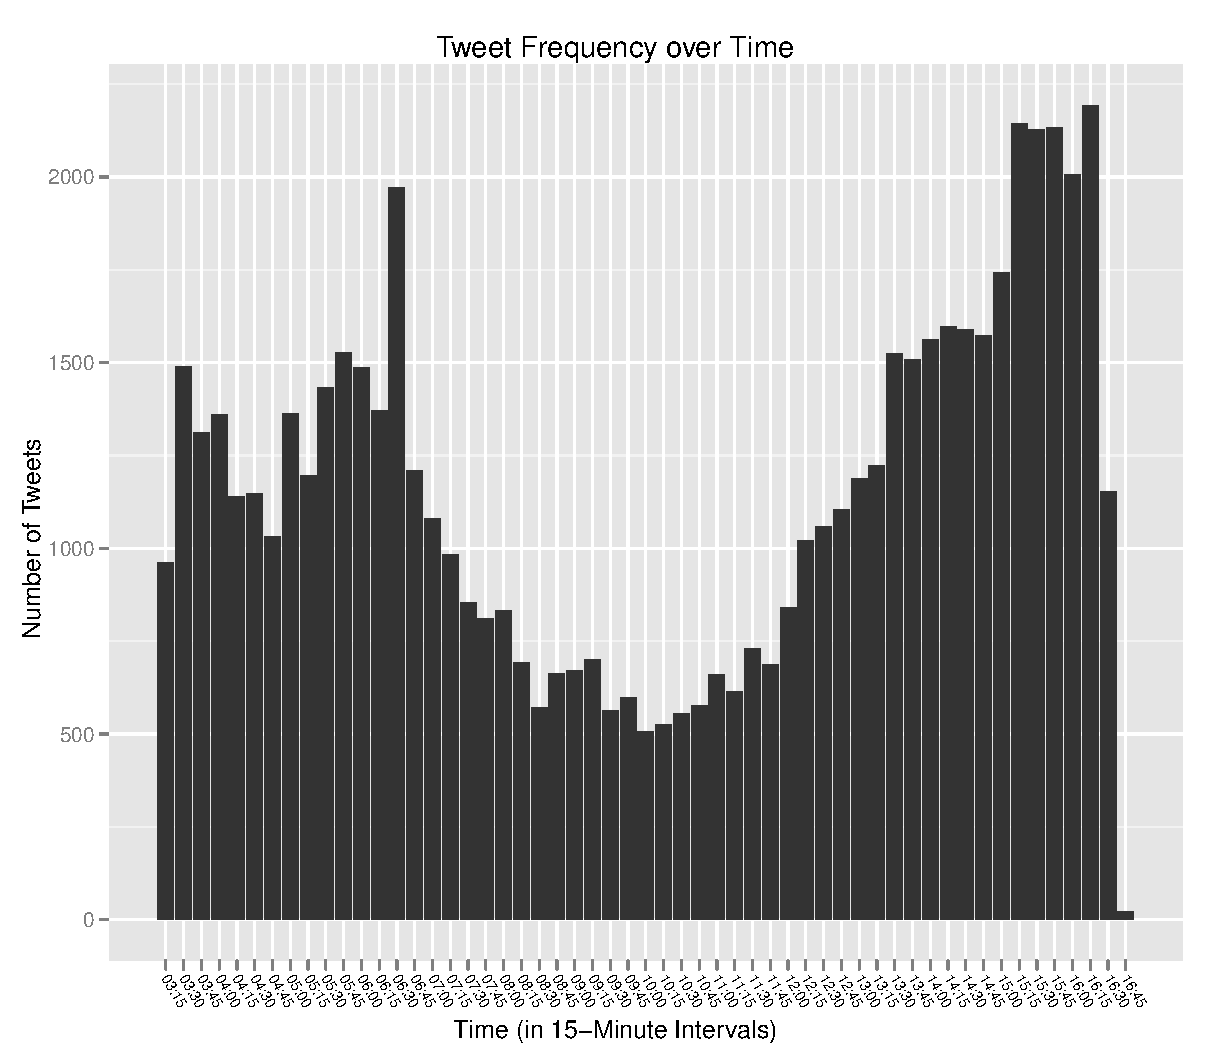
\includegraphics[width=120mm]{../figures/all_tweets_over_time}
\caption{All tweets over time.}
\label{fig:all_tweets_over_time}
\end{figure}

\begin{figure}[h]
\centering
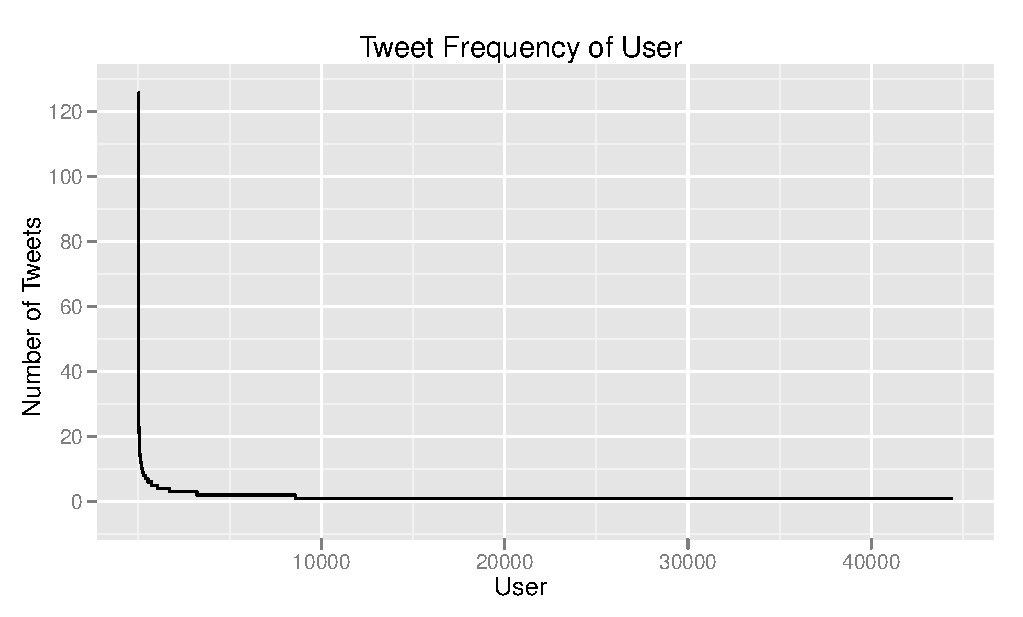
\includegraphics[width=120mm]{../figures/all_tweets_by_users}
\caption{All tweets over time..}
\label{fig:all_tweets_by_users}
\end{figure}

\begin{figure}[h]
\centering
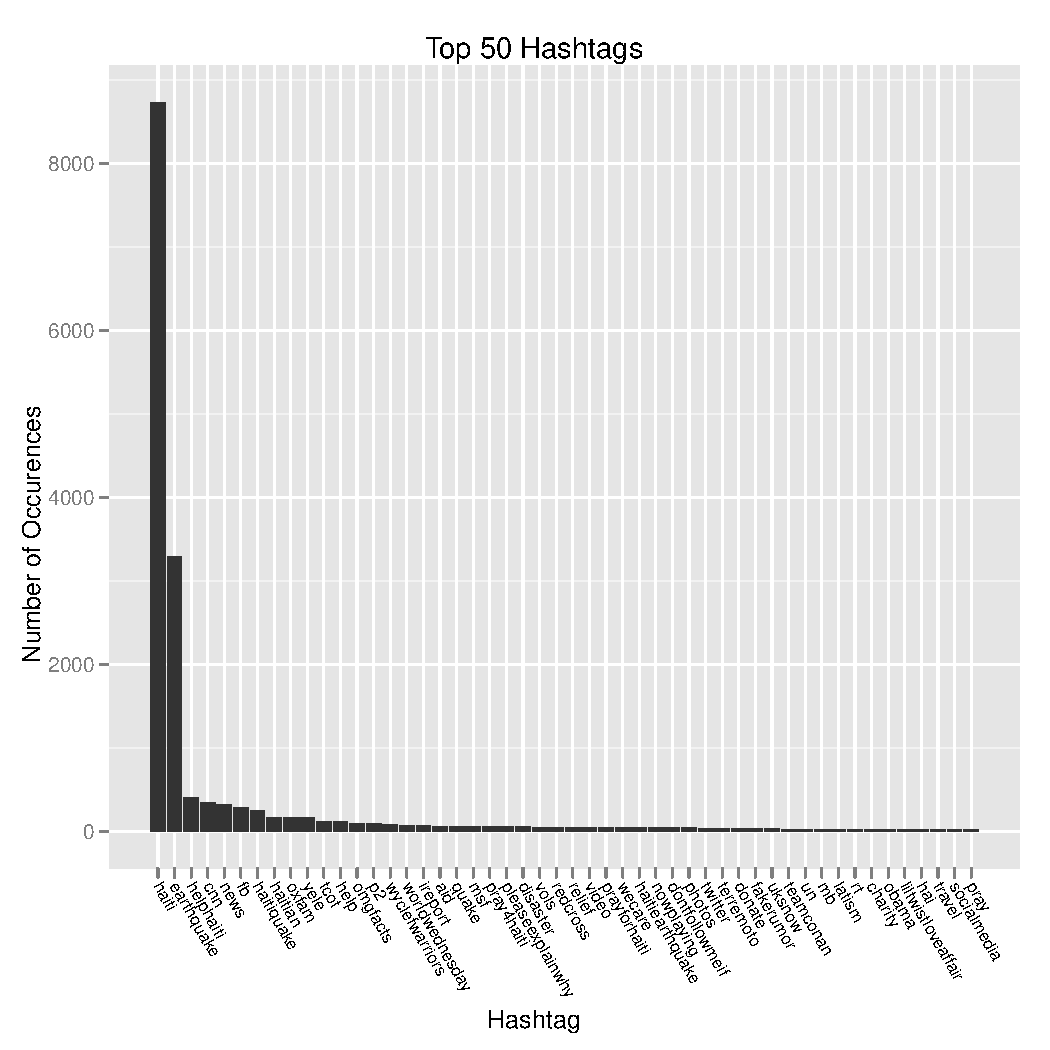
\includegraphics[width=\textwidth]{../figures/hashtag_counts.pdf}
\caption{Top 50 most common hashtags in our corpus.}
\label{fig:hashtag_counts}
\end{figure}

\section{Retweets}

Retweets account for 25\% of the collected messages from our corpus.  While there are 4,826 individual messages that were retweeted, only 4\% of those were retweeted 10 or more times.  Retweets provide evidence of user interaction and reaction are useful for determining the flow of information and user relationships.  We consider both the information diffusion and network relationships that may be inferred from analysis of the retweets in the dataset.

\subsection{Diffusion}

As shown in Figure~\ref{fig:rt_top_50}, \textit{iamdiddy}, the screen name of music artist Sean ``Diddy'' Combs was the author of the single most retweeted post.  There are 36 unique authors whose posts made it into the top 50; Wyclef Jean, CNN Breaking News, and LIFE.com had several posts each.  Wyclef Jean, a musician born in Haiti and nephew of the Haitian ambassador to the United States, had 11 posts in the top 50 with 5 of them in the top 10.  The Y\'{e}le Haiti Foundation, which Wyclef founded in 2005 to provide educational scholarships to Haitians, also had a top-50 retweet.  The top-50 list is unsurprisingly dominated by celebrities and popular media outlets.

\begin{figure}[h]
\centering
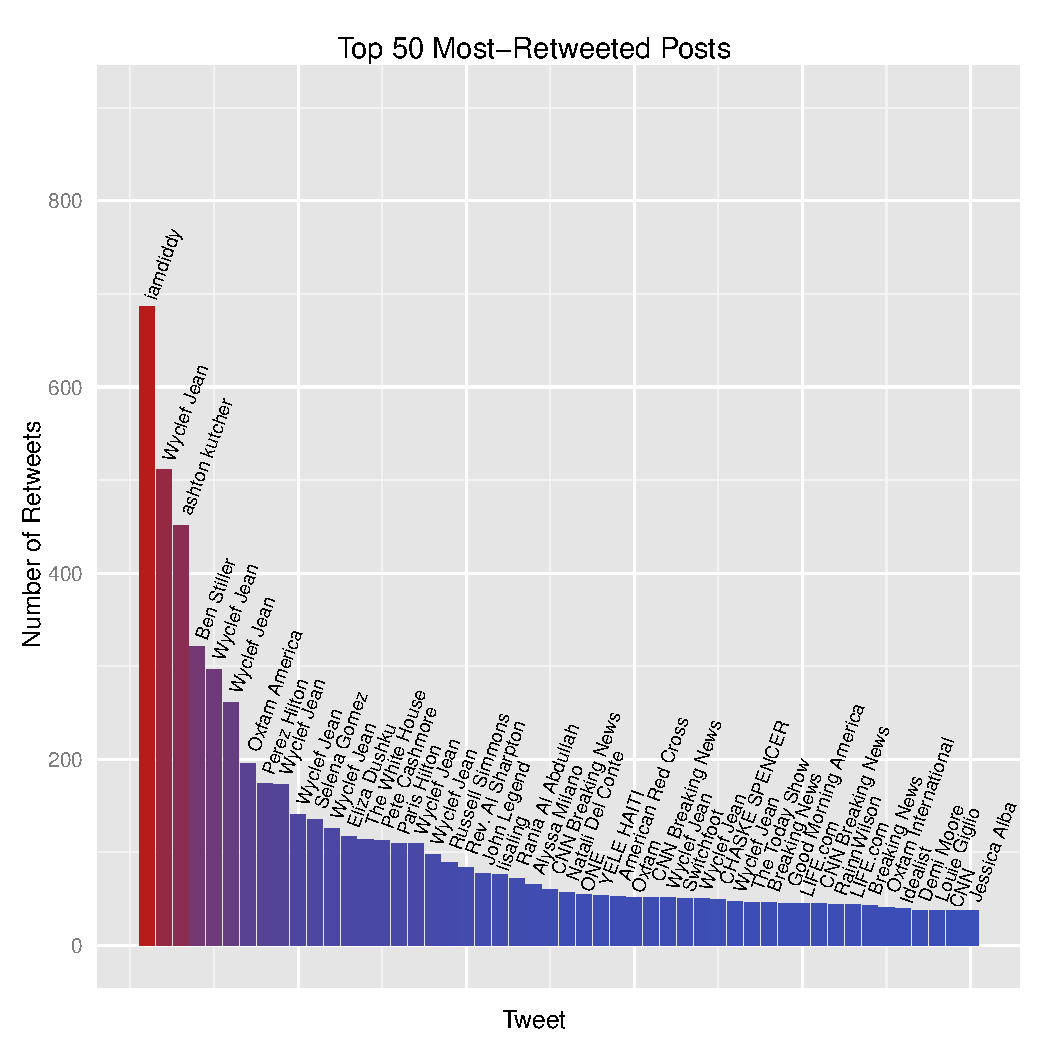
\includegraphics[width=120mm]{../figures/rt_top_50}
\caption{Top 50 most-retweeted posts.}
\label{fig:rt_top_50}
\end{figure}

\begin{figure}[h]
  \centering
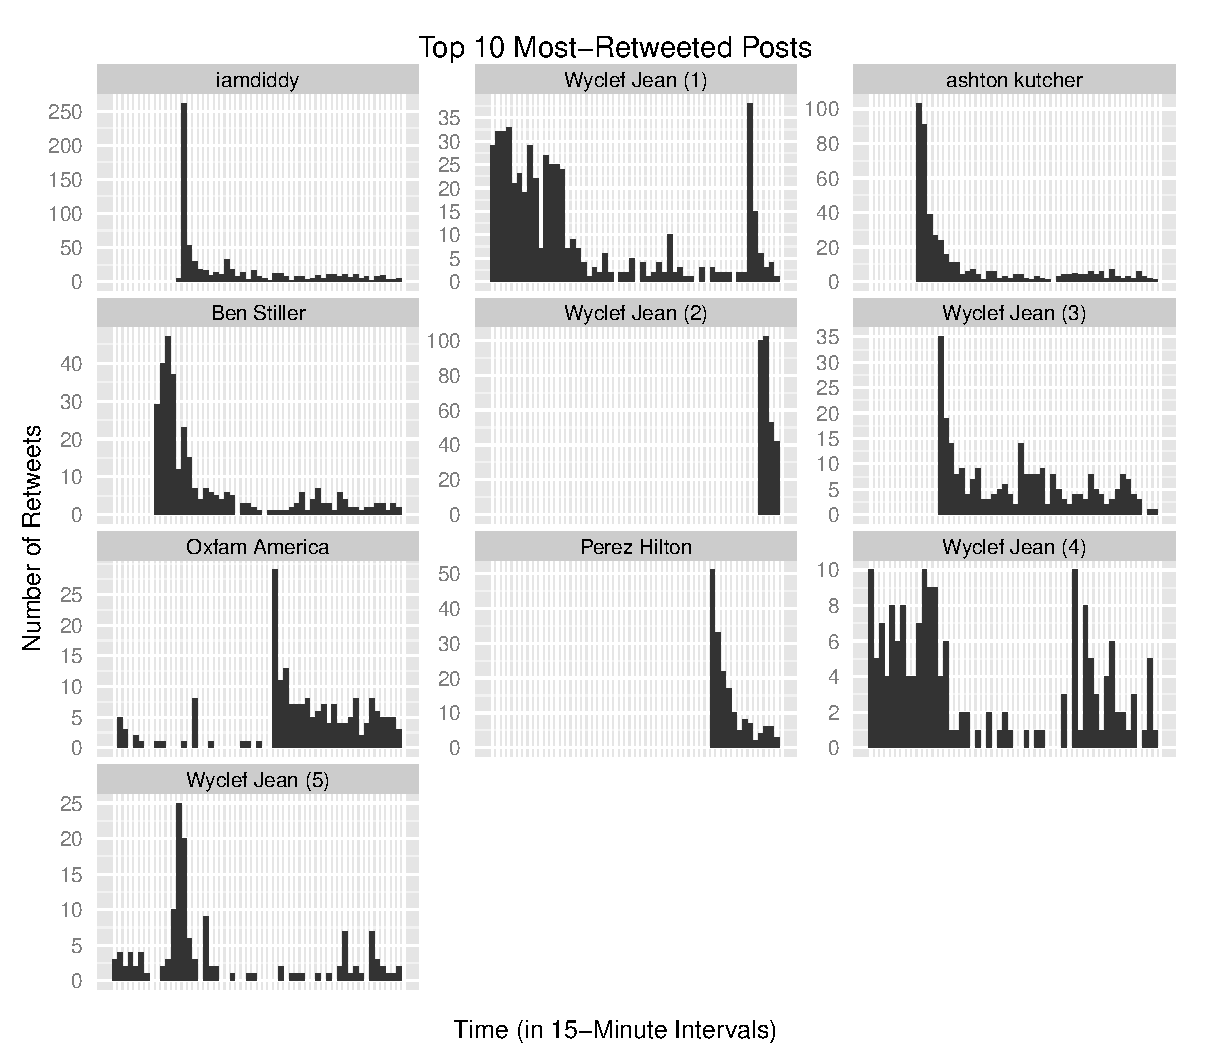
\includegraphics[width=120mm]{../figures/rt_top_10_over_time_free_scale}
\caption{Top 10 most-retweeted messages over time.}
\label{fig:rt_top_10}
\end{figure}

\begin{center}
  \begin{table}[!ht]
    \tiny{
  \begin{tabular}{| l | p{8.0cm} | c | c |}
    \hline
    \textit{Name} & \textit{Message} & \textit{Time} & \textit{\# Retweets} \\
    \hline
    iamdiddy & ``STATE OF EMERGENCY!!! RT PLEASE!!! Earthquake relief for Haiti please text YELE to 501501 to donate \$5 or go to www.yele.org RT PLS!!!'' & 06:29:20 & 687 \\
    \hline
    Wyclef Jean & ``Haiti is in need of immediate AID please text Yele to 510 510 and donate \$5 toward earthquake relief.'' & 02:53:08 & 511\\
    \hline
    ashton kutcher & ``If you want to DONATE to HAITI EARTHQUAKE RELIEF: http://tinyurl.com/ya6kpzm'' & 05:36:56 & 451 \\
    \hline
    Ben Stiller & ``If you want to DONATE to HAITI EARTHQUAKE RELIEF: http://tinyurl.com/ya6kpzm'' & 05:22:26 & 321 \\
    \hline
    Wyclef Jean & ``Haiti needs your help text YELE to 501 501 and 5 dollars will go toward earthquake relief.'' & 15:51:38 & 297\\
    \hline
    Wyclef Jean & ``Warriors Dontate to Earthquake relief in Haiti text Yele to  501 501 and visit www.yele.org'' & 06:35:11 & 261 \\
    \hline
    Oxfam America & ``Oxfam is already on the ground in \#Haiti after 7.0 magnitude earthquake hits. You can help now - please donate. http://bit.ly/8mrTkR'' & 01:57:01 & 196 \\
    \hline
    Perez Hilton & ``Another way you can help Haiti after their 7.0 earthquake: Donate \$5 by texting YELE to 501501 and by visiting www.yele.org'' & 13:34:10 & 174 \\
    \hline
    Wyclef Jean & ``Help Haiti Earthquake Relief Donate \$5 by texting YELE to 501 501 right now please RT'' & 01:33:23 & 173 \\
    \hline
    Wyclef Jean & ``Help Haiti Earthquake Relief Donate \$5 by texting YELE to 501 501 right now'' & 01:29:14 & 141 \\
    \hline
  \end{tabular}
    }
  \label{ref:top_retweets_table}
  \caption{The message's author, text, and time posted for the top 10 most-retweeted messages, sorted by number of retweets.  All times are in UTC and occurred on January 13.}
  \end{table}
\end{center}

As shown in Figure \ref{fig:rt_compare_over_time}, the fluctuation of retweet frequency during the night is similar to that of plain tweets.  Some users may elect to write original text and this could cause retweet and plain messages to similarly fluctuate.  Both retweet and plain message frequencies peak at 06:30, which corresponds to the posting of the most-retweeted message, authored by iamdiddy.  It is likely that some users elect to write original text or decline to credit the original author.  As morning begins in the Americas, the frequency of plain tweets grows faster than that of retweets.  This may be attributed to several factors, such as users receiving additional information from traditional media outlets and simultaneously introducing the news to Twitter.  

\begin{figure}[h]
\centering
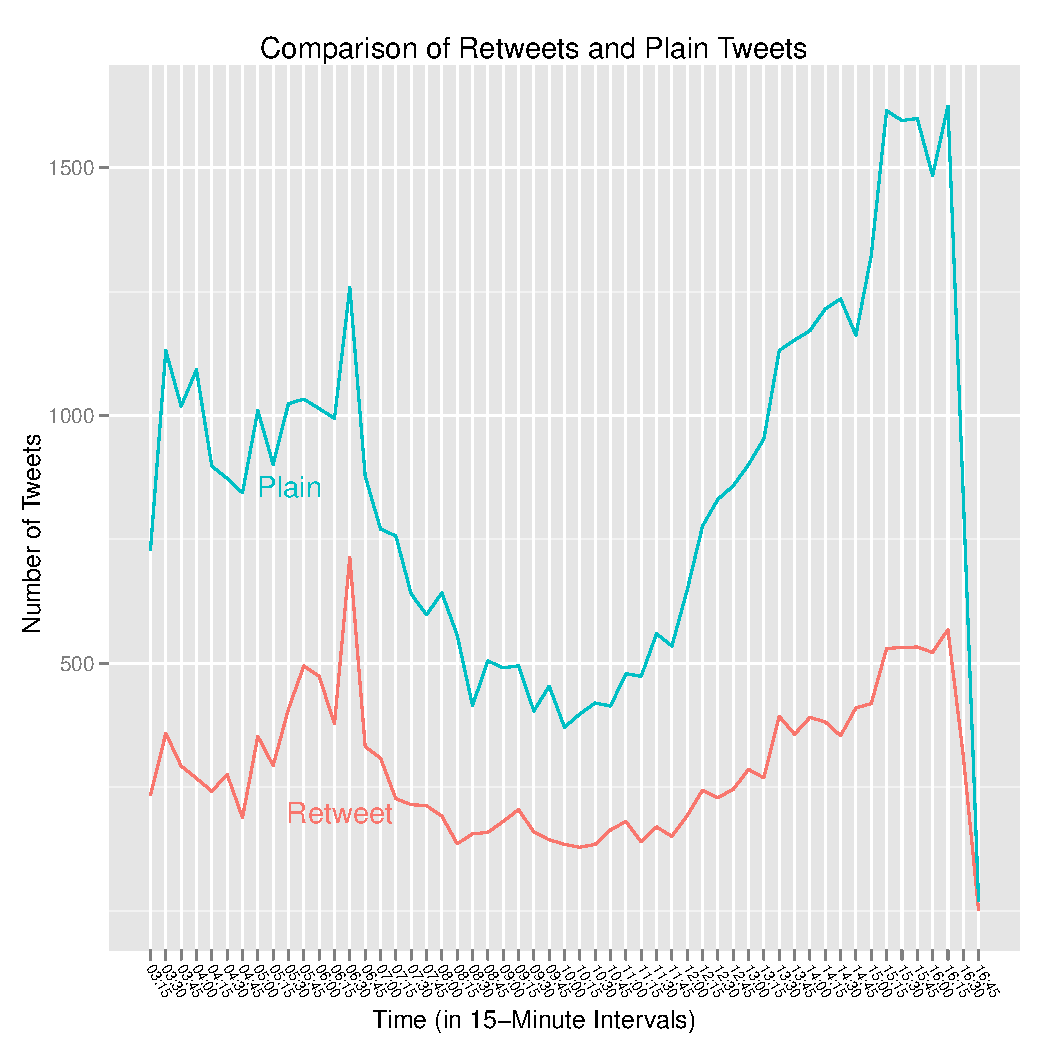
\includegraphics[width=120mm]{../figures/rt_compare_over_time}
\caption{Frequency of retweets compared to plain tweets over time.}
\label{fig:rt_compare_over_time}
\end{figure}

The most-retweeted message, by iamdiddy, peaks immediately after being published with over 250 users retweeting it in 15 minutes.  While many of the messages reach their apex shortly after posting, the popular Oxfam America message differs and doesn't peak until nearly 9 hours after it appeared.  The message was posted at 02:00 (9PM, EST) but mostly ignored until 10:50 (5:50AM, EST) when the band Coldplay resurrected it.

\subsection{Network}

Along with the dissemination of retweets, we considered a network of tweets related by which followers retweeted them.  This network, shown in Figure \ref{fig:rt_net_core}, uses shared audience as a relationship between retweeted messages.  The network consists of all retweeted messages as nodes and the existence of a common retweeter of any two messages as an edge.  For example, if a user retweets both iamdiddy's message and ashton kutcher's message, then those two messages are connected.  An edge weight is established By finding the total number of connections between two messages.  The constructed retweet network has a diameter of 10 and average clustering coefficient of 0.2715.

\begin{figure}[h]
\centering
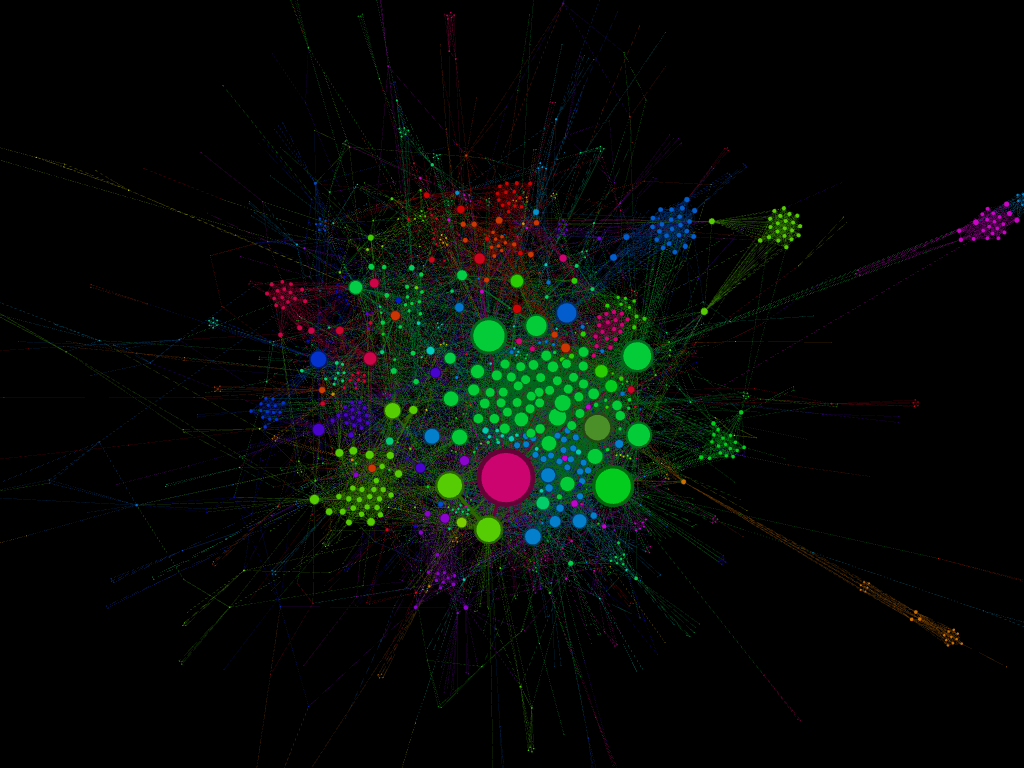
\includegraphics[width=120mm]{../figures/rt_net_core}
\caption{The core of the retweet network.}
\label{fig:rt_net_core}
\end{figure}

\begin{figure}[h]
\centering
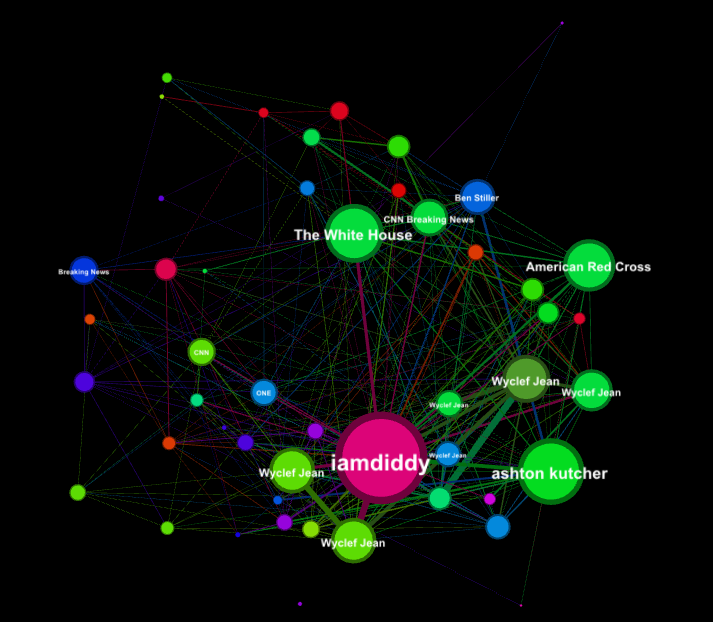
\includegraphics[height=90mm]{../figures/rt_net_top_50_labels}
\caption{Top 50 most-retweeted posts in the network.}
\label{fig:rt_net_top_50}
\end{figure}

Viewing only the top 50 most-retweeted messages (Figure \ref{fig:rt_net_top_50}) we see that heaviest edges are between Wyclef Jean's messages.  The post by iamdiddy is strongly-connected to Wyclef's message, but also the White House's and American Red Cross' posts.  There are two messages that are interesting outliers, the posts from Louie Giglio, the organizer of a Christian conference series, and Idealist, a community site for non-profits, are both disconnected from all top-50 messages.

\begin{figure}[h]
\centering
\label{fig:rt_net_core_clusters}
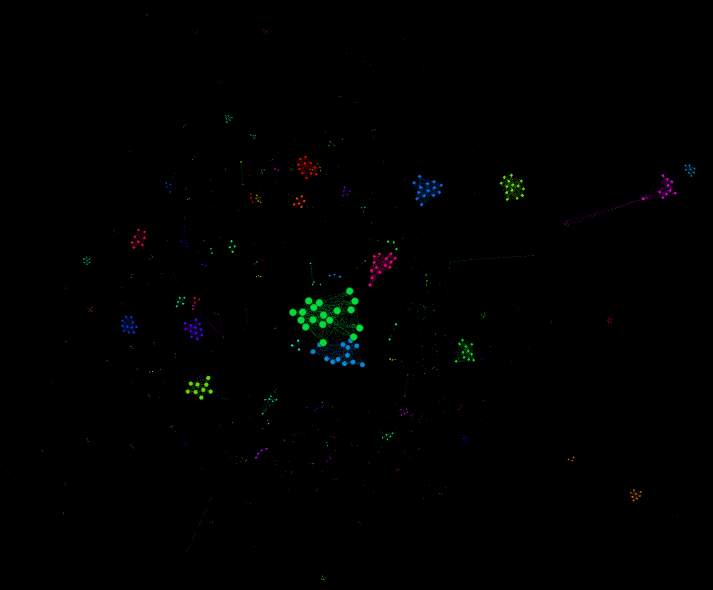
\includegraphics[width=90mm]{../figures/rt_net_core_clusters}
\caption{This is the network core, but with nodes filtered based on clustering coefficients.  By removing nodes with higher clustering coefficients we reveal the embedded tweet cliques.}
\end{figure}

\begin{figure}[h]
\centering
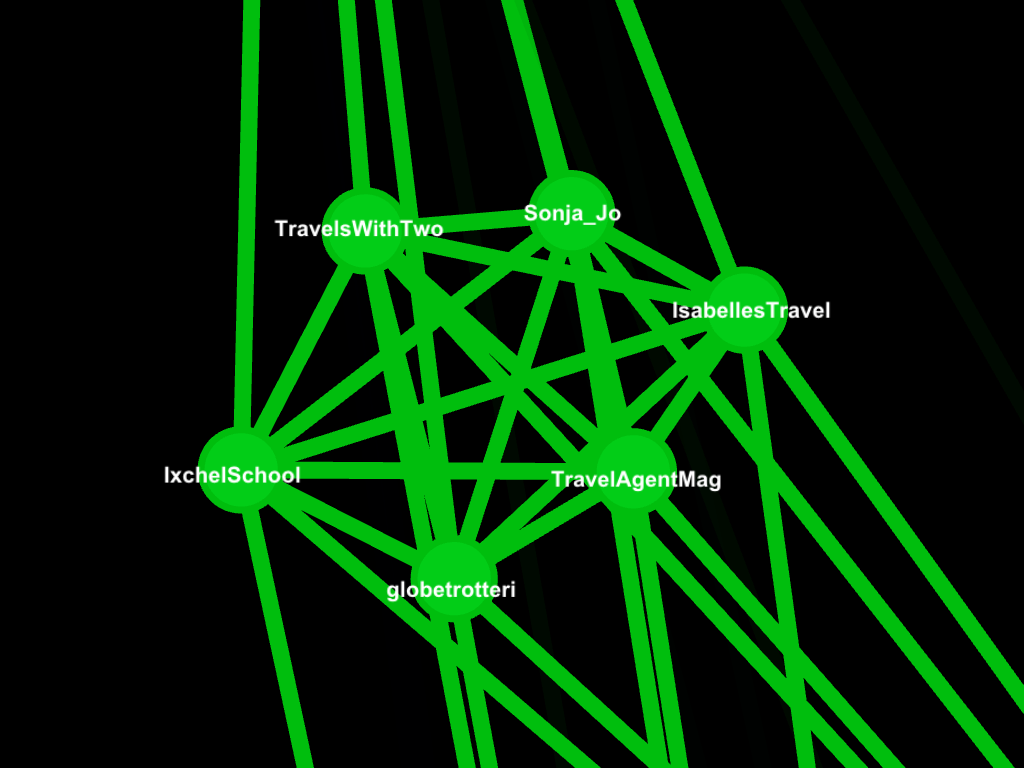
\includegraphics[width=90mm]{../figures/rt_net_travel}
\caption{A cluster of tweets from authors in the travel industry.}
\label{fig:rt_net_travel}
\end{figure}

In Figure \ref{fig:rt_net_travel}, a cluster of six messages is defined because a single user retweeted each of them.  This results in a clique of messages which suggests that the messages, or the original authors of the messages, have an external relationship.  In the case of this particular group, there are six, distinct authors and each is involved in the travel industry.  Rather than indicate a relationship between authors, some of the cliques found in the network group content.

\begin{figure}[h]
\centering
\subfloat[Two Clusters (red outline)]{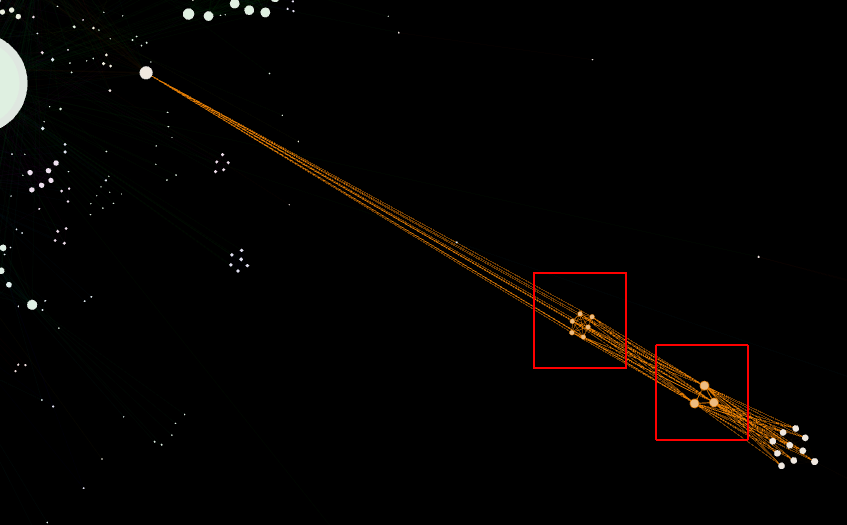
\includegraphics[width=60mm]{../figures/rt_net_photo_cropped_annotated}}
\quad
\subfloat[Boundary Spanner (red outline) and Two Clusters (blue outline)]{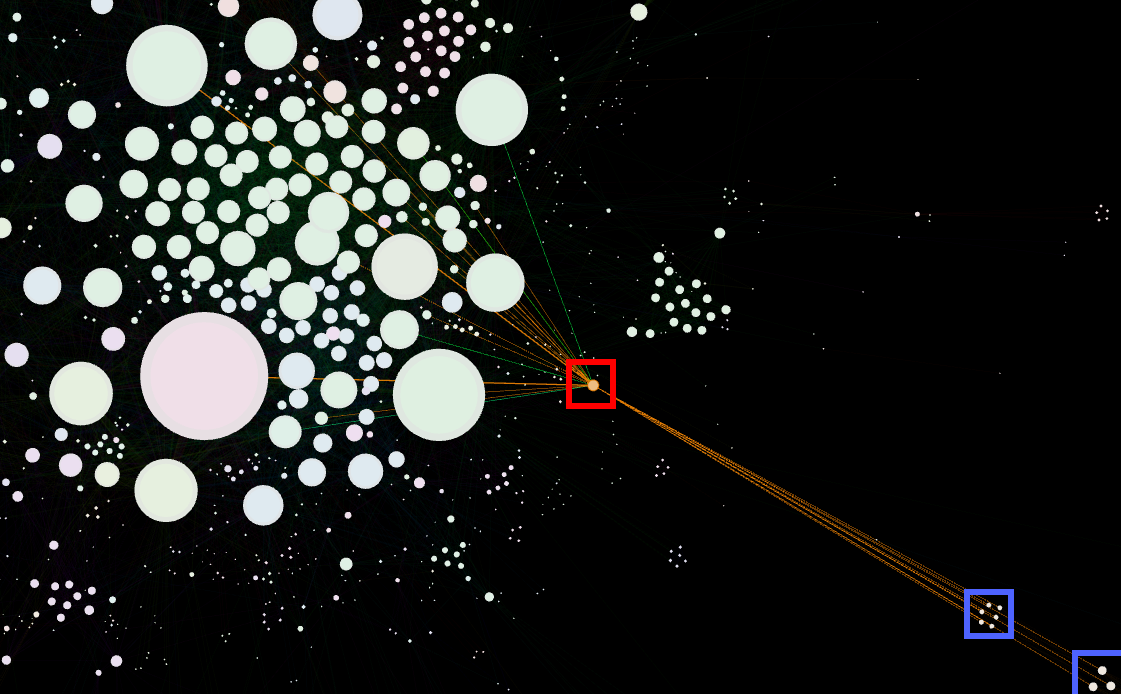
\includegraphics[width=60mm]{../figures/rt_net_photo_popular_annotated}}
\caption{Clusters of tweets representing sets of photos.}
\label{fig:rt_net_photos}
\end{figure}

\section{Hashtag Analysis}

A hashtag is any word prefixed by the ``\#'' symbol; they are used to refer to anything, including broad topics (e.g. Haiti, earthquake, news), organizations (e.g. Oxfam, Red Cross, World Concern, CBM), or even emotional sentiments (e.g. tragedy, dead, donate). The 50 hashtags mentioned most in our corpus are shown in Figure~\ref{fig:hashtag_counts}.



\begin{figure}[h]
\centering
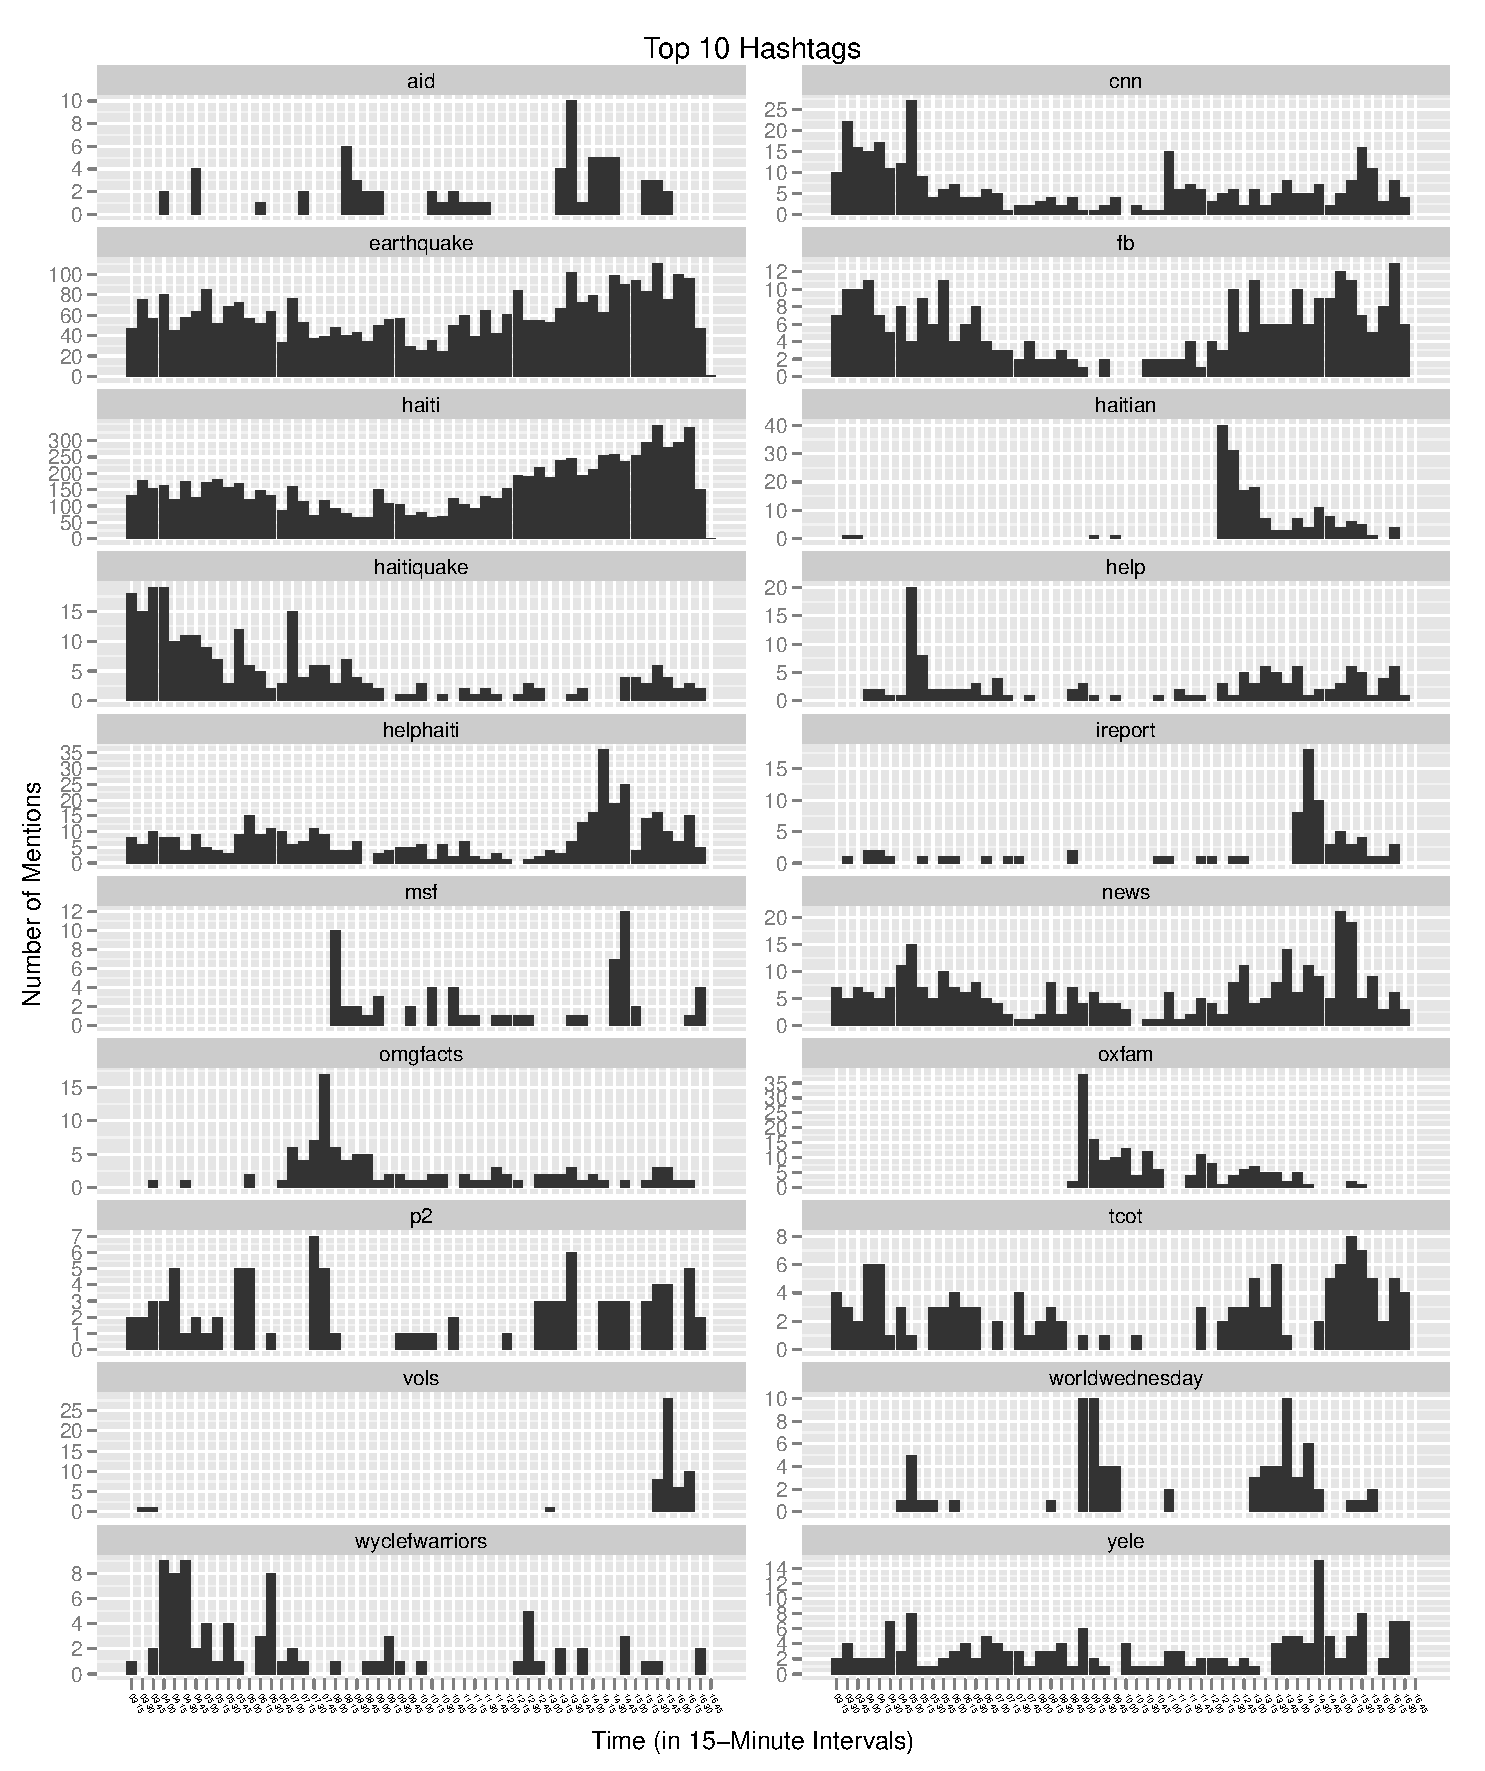
\includegraphics[width=\textwidth]{../figures/top-20-hashtags.pdf}
\caption{Top 20 hashtags over time. Note that the vertical axes vary in scale.}
\label{fig:hashtag_counts_over_time}
\end{figure}
\section{Conclusion}

Figure~\ref{fig:hashtag_counts_over_time} shows how different hashtags vary in frequency over time, revealing a number of interesting phenomena. The most-used hashtags, haiti and earthquake, vary with the typical daily ebb and flow of twitter activity, with a significant lull  between 3:00am and 6:00am EST. Some hashtags, such as \textit{\#haitian} and \textit{\#oxfam} see sharp spikes in use followed by an exponential decay. The resurgence of \textit{\#oxfam} corresponds to the retweet by Coldplay mentioned above.

The hashtag \textit{\#haitiquake} is interesting in that it declines steadily over time. This is apparently one tag which didn't catch on.

\subsection{Group Network}

To find relationships between different hashtags we built the ``group network'', in which each node represents a unique hashtag and each edge represents the fact that an author mentioned both hashtags (though not necessarily in the same tweet). The \textit{weight} of an edge represents the number of authors who mentioned the pair of tags connected by the edge. For example, \textit{\#earthquake} was mentioned 3,299 times by 2,329 different authors; \textit{\#haiti} was mentioned 8,729 times by 6,597 different authors; and 1,994 different authors mentioned both tags. Thus, the edge $\textit{\#earthquake}~\leftrightarrow~\textit{\#haiti}$ has weight of 1,994. The degree distribution is long tailed with many hashtags sharing a single link or pair of links, and very few hashtags containing a large number of shared links. Figure~\ref{fig:ht_group_network} shows the group network, filtered to remove edges with a weight of less than 3, then nodes with a degree of less than 3. Filtering based on these parameters is highly effective at isolating and eliminating self-promotional spam cliques.

\begin{figure}[h]
\centering
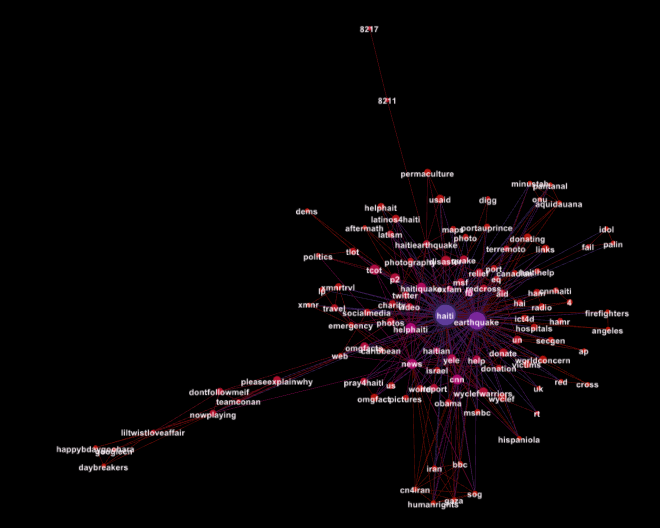
\includegraphics[width=0.5\textwidth]{../figures/ht_group_network}
\caption{Hashtag group network, filtered to remove edges with a weight of less than 3, then nodes with a degree of less than 3. }
\label{fig:ht_group_network}
\end{figure}

\subsection{Hashtag Ego Networks}
During the time window during which our corpus was collected, there were many requests for aid both by, and on behalf of, international relief organizations. By isolating different hashtag ego networks we see some semantic clustering of terms. Figure~\ref{fig:ht_ego_graphs} shows the ego graph of the hashtags \textit{\#donate}, \textit{\#oxfam}, \textit{\#redcross}, and \textit{\#cbm}. 




\begin{figure}[h]
\centering
\subfloat[\textit{\#donate} ego network]{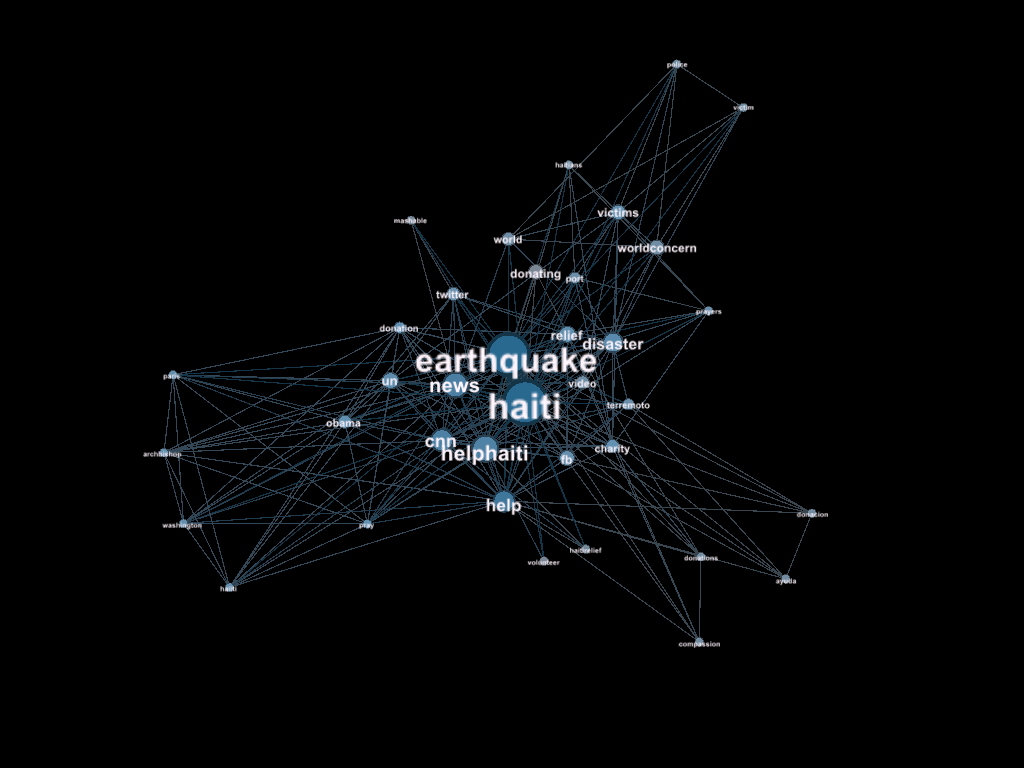
\includegraphics[width=60mm]{../figures/ego_donate}}
\quad
\subfloat[\textit{\#oxfam} ego network]{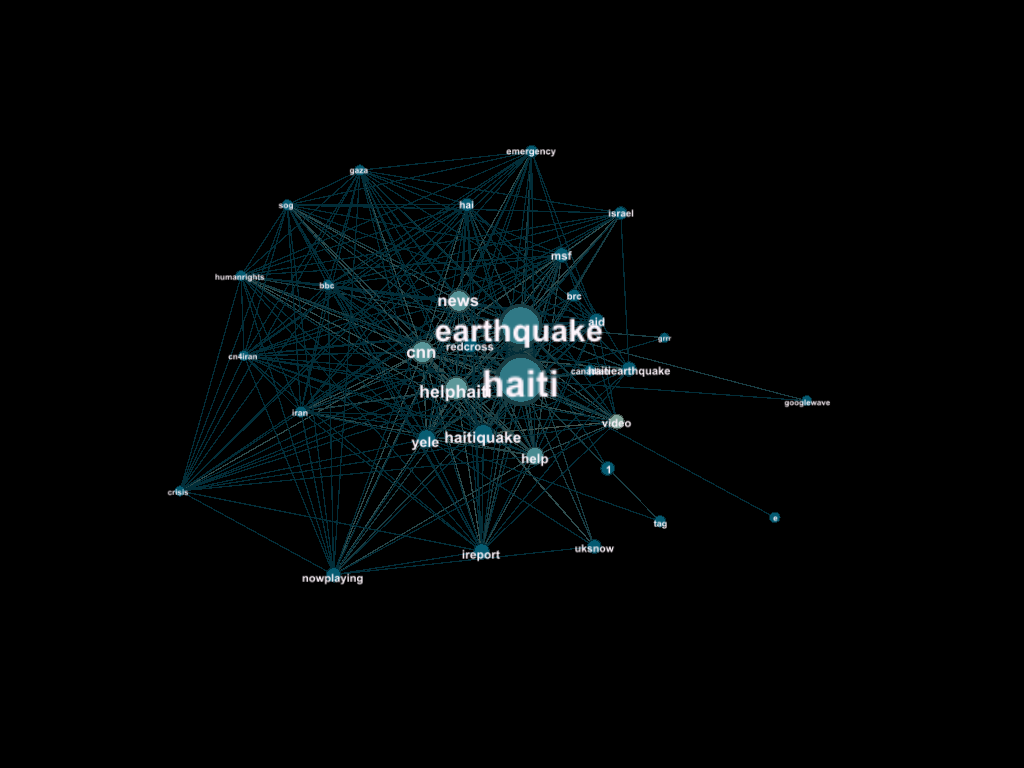
\includegraphics[width=60mm]{../figures/ego_oxfam}}
\quad
\subfloat[\textit{\#redcross} ego network]{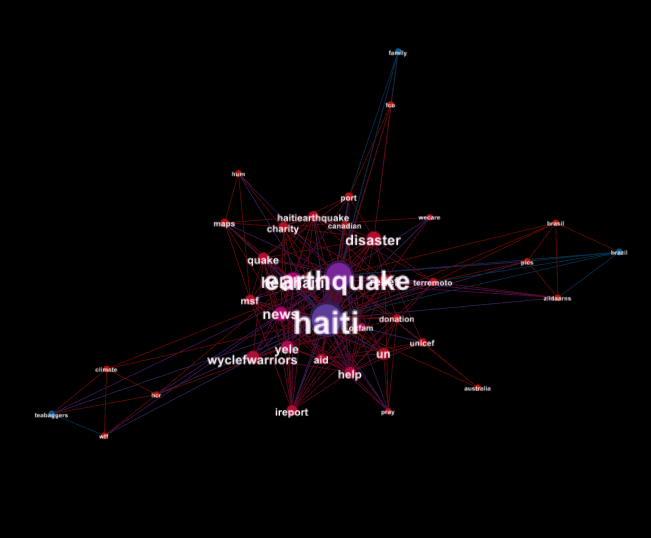
\includegraphics[width=60mm]{../figures/ego_redcross}}
\quad
\subfloat[\textit{\#cbm} ego network]{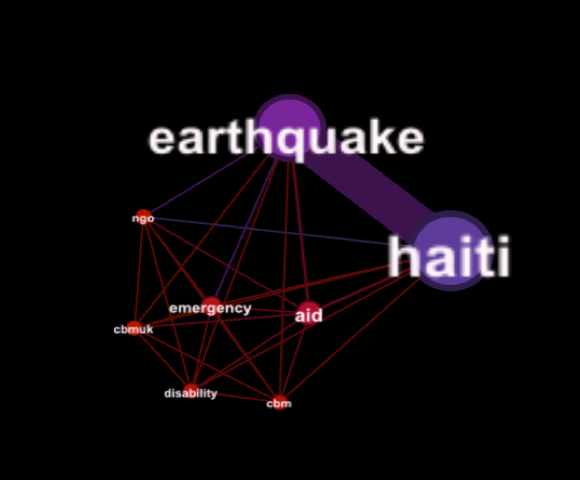
\includegraphics[width=60mm]{../figures/ego_cbm}}
\quad
\caption{Ego networks for some charity-related hashtags. There are more popular hash}
\label{fig:ht_ego_graphs}
\end{figure}



%Sentiments:
%tragedy
%donate
%dead



Though our corpus only provided us with data covering a 13-hour time span, it was enough to offer a glimpse at how Twitter users respond to breaking news and emergencies.  Some findings are expected given certain assumptions.  For example, if we assume that the majority of active Twitter users are in the United States, the drop in posting frequency which corresponds to nighttime in the Americas is expected.  The formation of meaningful cliques in the retweet network is the most unexpected result.  Cliques of messages, such as those posted by individuals in the travel industry or the images captured by the photographer, group related material

\section{Acknowledgements}

The analysis and figures produced for this paper would not have been possible without R\cite{R}, ggplot2\cite{wickham2008ggplot2, wickham2009ggplot2}, and Gephi\cite{bastian2009gephi}.
The old testament of network analysis, \cite{wasserman1994sna}, was used as a reference.

\bibliographystyle{splncs}
\bibliography{bibfile}

\end{document}
